\subsection{Objectif}
%on cherche a ne pas utiliser la kinect
Cette première application a plusieurs objectifs. Dans un premier temps, nous souhaitons réaliser 
une segmentation sans utiliser les outils fournis pas la Kinect, dans le but d'obtenir une méthode plus
précise ou, tout du moins, permettant d'améliorer une partie du procédé de segmentation. Comme nous l'avons vu dans 
l'état de l'art, les méthodes utilisées par la Kinect ont évolué et sont devenues plus stables et plus précises.
Le second objectif est de remplacer un nuage de points représentant un membre par un modèle 3D de ce même membre
mais ayant une forme différente. Cette première partie du stage me permet surtout d'aborder des concepts qui me 
serviront dans la seconde application qui est le but premier de ce stage.

\subsection{Délimitation du corps humain et minimisation de la quantité de donnée}
Durant cette première phase, nous travaillons sur un nuage de points et non sur les informations de l'image de profondeur.
Comme nous l'avons dit précédemment, l'ensemble des informations n'est pas pértinente pour les traitements que nous souhaitons
réaliser. La première étape dans la réalisation de cette application est de supprimer l'ensemble des informations qui ne se rapportent pas 
au corps humain. La première solution que nous développons consiste à utiliser deux seuils. Les points qui sont plus éloignés que le 
premier seuil, ainsi que les points en dessous du second seuil sont supprimés. 
Ces seuils sont les distances, en mètre, dans lequel l'utilisateur doit se trouver. Cette méthode est utilisée dans 
l'application ReconstructMe\footnote{\url{http://reconstructme.net}} qui est une application permettant de construire un modèle
3D complet à partir de données fournies par plusieurs images provenant d'une caméra 3D. Comme pour cette application, nous avons
décidé de laisser la possibilité à l'utilisateur de changer les seuils en fonction de son besoin.\\

\begin{figure}[!ht]
  \begin{center}
    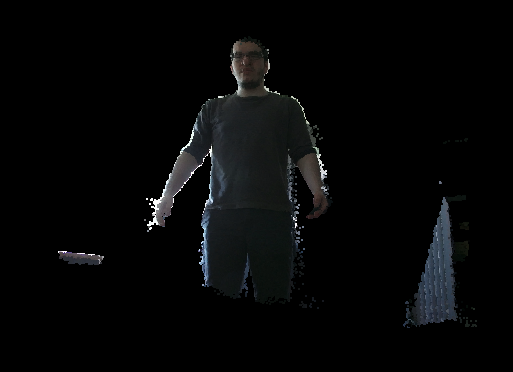
\includegraphics[width=8cm]{image/seuil1.PNG}
    \caption{Résultat d'une segmentation par seuillage}
    \label{fig:seuillage}
  \end{center}
\end{figure}

Nous pouvons voir sur la Fig. \ref{fig:seuillage} que le seuil permet effectivement de supprimer beaucoup d'informations
correspondant à l'environnement, mais qu'il reste beaucoup de bruit dû à la qualité de l'acquisition de la caméra ainsi que 
des objets qui se trouvent à la même distance que l'utilisateur. La librairie
PCL\cite{PCL} nous fournit beaucoup d'outils pour ce genre de problèmatique. Il y a une classe appelée \textit{StatisticalOutlierRemoval}
qui permet de supprimer les points supposés être du bruit. Pour cela, cette classe calcule la distance moyenne d'un point avec son
voisinage et si cette moyenne est trop élevée, elle supprime le point en question. Cependant, l'utilisation de cette classe ne
suffit pas à supprimer les objets à la même distance que l'utilisateur, car la densité de points de ces objets leur permet d'avoir
suffisamment de voisins proches pour avoir une moyenne de distances très petites. Pour pallier à ce problème, nous avons ajouté un
système de sélection permettant à l'utilisteur de sélectionner les données ne faisant pas partie du corps humain.\\

Pour la suite des traitements que nous souhaitons réaliser, il est préférable d'avoir un minimum d'informations et de ne garder
que ce qui est pertinent. Le corps humain que nous avons réussi à délimiter comporte encore beaucoup trop de données. Le nombre
de points fourni par la Kinect est très important et très concentré, il est possible de supprimer des points qui sont trop 
proches les uns des autres. Là encore PCL\cite{PCL} peut nous aider avec la classe \textit{VoxelGrid}. Cette classe crée une grille de
voxels sur le nuage de points, dont la taille est définie par l'utilisateur. L'ensemble des points, à l'intérieur d'un voxel, sont 
approximés en un point qui correspond au centroïde du voxel. Grâce à l'ensemble de ces traitements, nous ne gardons que l'information 
essentielle à nos traitements.

\subsection{Calcul de la distance géodésique}
Notre première idée pour segmenter le corps humain est d'utiliser la distance géodesique. Y. Liu et al\cite{GIF} montre que la distance
géodesique pour une même personne, quelque soit sa posture, est toujours la même pour les points de ses membres. Le seul problème 
est que plusieurs membres ont la même distance géodésique, on ne peut donc pas associer un membre directement à une distance.
Cependant, il est possible de seuiller le corps et de calculer des descripteurs, afin de déterminer quel nuage de points
correspond à quel membre.\\

Avant de calculer la distance géodésique du corps humain, nous avons besoin de créer un maillage sur le nuage de points. Pour cela,
j'ai repris le principe utilisé pour le descripteur FPFH\cite{FPFH} pour la sélection des voisins. Dans un premier temps, je calcule
la distance euclidienne de chacun des points du nuage de points avec tous les autres. Pour la création du voisinage, nous considérons non
seulement le nombre maximum de points à prendre en compte, mais aussi la distance maximum d'un point avec les autres. Nous avons eu
de nombreux problèmes lorsque nous n'avions pas mis la seconde condition, car lorsque la main de l'utilisateur était trop proche de sa 
jambe, certains points de la main avaient des voisins dans la jambe. Cette partie de l'algorithme est la plus délicate, car nous ne pourrons
pas avoir un aussi bon maillage que sur un modèle 3D et la distance géodésique repose sur la qualité de celui-ci. Pour l'améliorer, nous avons créé deux paramètres que l'utilisateur peut modifier. Le premier paramètre est le nombre de voisins d'un point et
le second est la distance euclidienne maximale entre les voisins.\\

%TODO voir si on met des exemples de maillage defectueux 

A cette étape de l'algorithme, nous avons donc un maillage et les distances euclidiennes de chaque point avec son voisinnage. Pour calculer
la distance géodésique du centroïde du nuage de points avec chaque point, nous allons utiliser l'algorithme de Dijkstra\cite{dijkstra}.
Il faut donc trouver le plus court chemin du centroïde jusqu'au point dont on veut calculer la distance géodésique, en passant par le
maillage que nous avons construit précédemment. Les valeurs prises en compte entre chaque point dans l'algorithme de Dijkstra seront
les distances euclidiennes entre les points. A chaque fois qu'un point est ajouté au chemin emprunté par l'algorithme il faut 
additionner la distance euclidienne entre ce point et le précédent, pour obtenir un résultat final correspondant à la distance 
géodésique entre le centroïde et le point dont on cherche la distance.\\

\begin{figure}[!ht]
  \begin{center}
    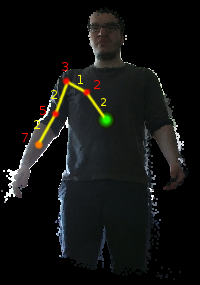
\includegraphics[width=5cm]{image/cheminGeodesique.PNG}
    \caption{Exemple de chemin parcouru par l'algorithme de calcul de la distance géodésique pour un point.
    Le point vert correspond au centre de gravité du corps, les points rouges sont les noeuds du chemin et le point 
    orange est le point d'arrivée. Les chiffres jaunes sont les distances pour aller d'un noeud à l'autre, et les chiffres
    rouges sont la distance géodésique au noeud correspondant.}
    \label{fig:cheminGeodesique}
  \end{center}
\end{figure}

\begin{figure}[!ht]
  \begin{center}
    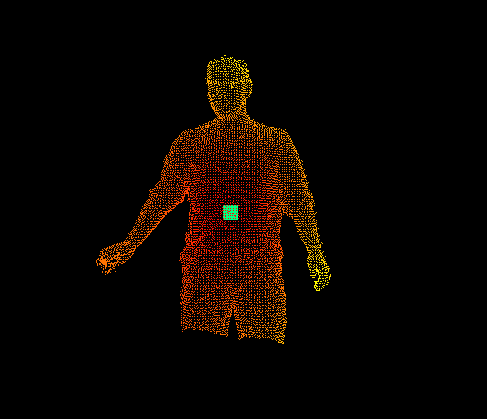
\includegraphics[width=6.5cm]{image/geodesic1.PNG}
    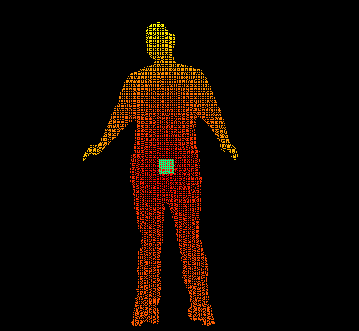
\includegraphics[width=6cm]{image/geodesic2.PNG}
    \caption{Résultat du calcul de la distance géodésique sur l'ensemble du nuage de points. Le point vert correspond au centroïde du
    nuage de points. Plus la couleur des points est proche du rouge, plus les points sont proches du centroïde.}
    \label{fig:geodesique}
  \end{center}
\end{figure}

Sur les images de la Fig. \ref{fig:geodesique}, on peut voir que la distance géodésique n'est pas aussi précise qu'on le souhaiterait.
Dans la première image, on voit que la distance géodésique n'est pas la même sur le bras gauche et sur le bras droit. Cette imprécision
vient de la qualité du maillage. Certains points ne passent pas par le corps et traversent dans le vide du ventre au bras, ce qui réduit
la distance géodésique au niveau des mains. Dans la seconde image, on voit que la position du centroïde est très importante. Celle-ci change en fonction de ce que l'on voit du corps humain, ce qui modifie également la distance géodésique. Un simple seuillage
n'est donc pas suffisant pour segmenter le corps humain, car de trop nombreux paramètres interviennent dans le calcul de la distance géodésique,
y compris la physionomie de l'utilisateur.

\subsection{Segmentation du corps humain}
%recherche du point le plus éloigné puis suppression d'un groupe de point ....
%voir si on parle des superpixels
Malgré un léger manque de précision de la part du calcul de la distance géodésique sur le corps humain, nous avons testé une
méthode de segmentation qui ne prend pas en compte cette imprécision. Le principe de cette segmentation est de détecter le
membre le plus éloigné, puis de le supprimer dans la recherche des autres membres. Pour cela, notre algorithme recherche le point
dont la distance géodésique est la plus grande et forme une zone autour de ce point. Cette zone a un rayon prédéfini qui sera le 
même pour chaque membre. Les points à l'intérieur de cette zone seront enregistrés et sont considérés comme faisant partie d'un 
même membre. Ils seront ensuite supprimés du nuage de points du corps humain, afin de ne pas être pris en compte dans les 
étapes suivantes.\\

\begin{figure}[!ht]
  \begin{center}
    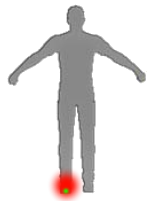
\includegraphics[width=3cm]{image/humanFootR.png}
    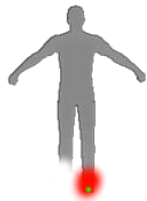
\includegraphics[width=3cm]{image/humanFootL.png}
    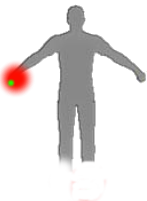
\includegraphics[width=3cm]{image/humanHandR.png}
    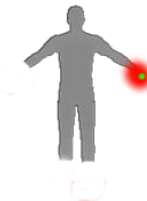
\includegraphics[width=3cm]{image/humanHandL.png}
    \caption{Premières étapes de l'algorithme de segmentation du corps humain. Le point vert correspond au point le plus éloigné et la zone rouge correspond à
    l'ensemble des points considérés comme faisant partie du membre.}
    \label{fig:segmentation}
  \end{center}
\end{figure}

Y. Liu et al\cite{GIF} proposent une amélioration de leur méthode basée sur le superpixel SLIC\cite{SLIC}. Le but de l'utilisation du superpixel
SLIC est de diminuer le nombre de points pris en compte lors des calculs du plus court chemin de l'algorithme de Dijkstra afin de diminuer le 
temps de calcul. Cela permet également d'améliorer la segmentation du corps humain. Le seul paramètre de l'algorithme SLIC est le nombre de classe à 
retrouver dans l'image. Cet algorithme s'effectue en général dans l'espace colorimètrique LAB. La méthode de Y. Liu et al\cite{GIF} quant à
elle, utilise les coordonnées x, y et z. Après avoir testé l'utilisation des superpixels, nous remarquons que nous obtenons plus rapidement le résultat,
mais que celui-ci n'est pas meilleur que celui que nous obtenions précédemment.\\

%TODO mettre une image avec les superpixel en rouge
%TODO faire une comparaison entre les résultats obtenu avec et sans les superpixel

Cette méthode est efficace pour reconnaitre les extrémités du corps humain comme les mains, les pieds et la tête. Le reste des parties du corps 
est moins précis, notamment au niveau des épaules où le point de la zone est très instable et peut se retrouver au niveau du torse. De plus, la taille 
des zones dépend de la physionomie de la personne devant la Kinect. 

\subsection{SDK de la Kinect}
Etant donné que nos résultats pour la segmentation du corps ne sont pas suffisamment précis pour la suite de nos traitements et par faute de
temps, nous avons décidé d'utiliser les outils fournis avec la Kinect pour continuer le projet. Grâce à la caméra de Microsoft, nous pouvons
récupérer le squelette de l'utilisateur dont les articulations sont labellisées avec le nom de la partie du corps humain à laquelle elle appartient
(voir Fig. \ref{fig:kinect}.a). De plus, la Kinect nous permet de séparer les points qui appartiennent à l'utilisateur de ceux qui appartiennent
à l'environnement (voir Fig. \ref{fig:kinect}.b).\\

\begin{figure}[!ht]
  \begin{center}
    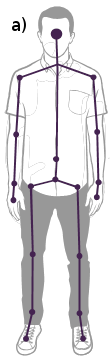
\includegraphics[width=2cm]{image/kinectSkeleton.png} 
    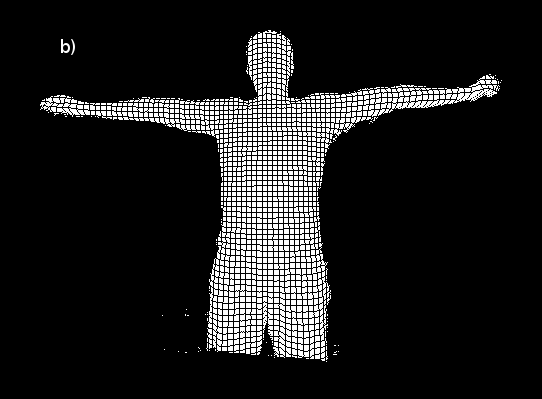
\includegraphics[width=8cm]{image/seg1.PNG}
    \caption[The LOF caption]{a) Squelette fourni par la caméra Kinect\footnotemark et b) séparation du corps humain de l'environnement}
    \label{fig:kinect}
  \end{center}
\end{figure}
\footnotetext{source : \url{http://hdimagelib.com/standing+person+sideways?image=356490844}}

Grâce à ce squelette et au nuage de points, nous pouvons segmenter le corps humain. Pour cela, pour chaque articulation nous définissons une zone
dont la taille est variable en fonction de l'articulation. Les points du nuage sont labellisés en fonction de leur distance avec les articulations.
Donc, un point prend le label de l'articulation dont il est le plus proche.\\

\begin{figure}[!ht]
  \begin{center}
    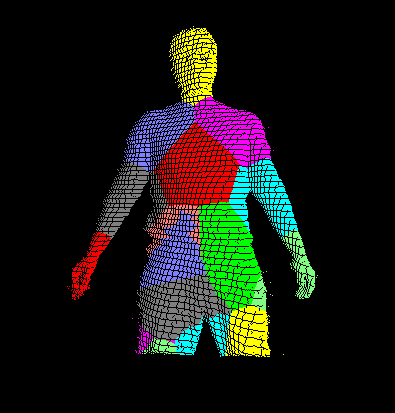
\includegraphics[height=4cm]{image/lab1.PNG} 
    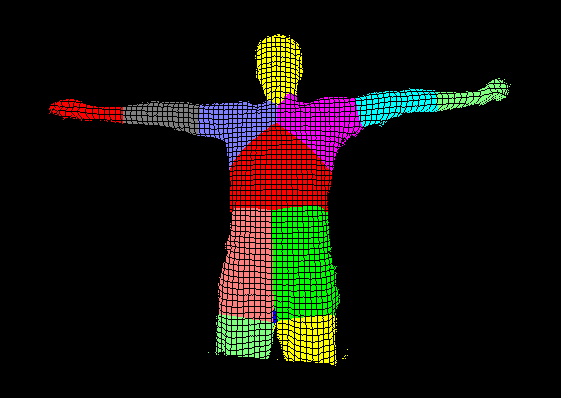
\includegraphics[height=4cm]{image/lab2.PNG}
    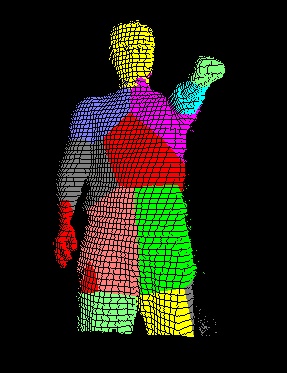
\includegraphics[height=4cm]{image/lab3.PNG}
    \caption{Résultat obtenu avec la segmentation du corps humain via les outils de la Kinect}
  \end{center}
\end{figure}

Nous pouvons voir que comme nous l'attendions, le résultat de cette segmentation est bien meilleur puisque nous avons à notre disposition
beaucoup plus d'informations qu'auparavant grâce au squelette de l'utilisateur. Même si cette segmentation n'est pas parfaite, comme on peut
le voir dans la première image, elle reste suffisante pour nos futurs traitements. En plus de la segmentation, nous connaissons déjà le nom
des membres grâce aux labels des articulations. Nous n'avons donc pas besoin de passer par une étape de reconnaissance des parties du
corps, car celle-ci a déjà été réalisée par les outils de la Kinect. Il ne reste plus qu'à supprimer le bruit présent dans les membres, les points
mal labelisés, grâce à la classe StatisticalOutlierRemoval que nous avons vu précédemment.

\subsection{Positionnement}
La dernière étape de cette première application est d'échanger le nuage de points d'un membre du corps par un modèle 3D représentant cette même partie
du corps. Cette étape est très complexe à cause de deux problèmes majeurs. Tout d'abord, le type d'information n'est pas le même. Dans un cas, nous avons
un nuage de points dont les points sont très concentrés, mais avec des parties occultées. De l'autre côté, nous avons un modèle 3D avec un nombre de points
inconnus, donc une concentration de points inconnu, mais sans zone occultée si nous prenons en considération le maillage du modèle. Le second problème
est que le but recherché est de remplacer la partie du corps humain par quelque chose de plus improbable et étonnant comme une partie du corps d'un monstre,
d'un robot ou d'un corps dont la musculature est différente.\\

Nous testons dans un premier temps l'algorithme le plus utilisé dans la littérature en terme de correspondance de modéle 3D. L'algorithme ICP\cite{ICP} est
disponible dans la librairie PCL\cite{PCL}. Après plusieurs tests sur différentes parties du corps, nous pouvons voir que l'algorithme ICP arrive à déterminer
la bonne translation, si on compare les centroïdes des modèle 3D avec leur partie du corps correspondant. Cependant, ICP ne parvient pas à déterminer
l'orientation du modèle. Le problème vient du fait que les données ne sont pas les mêmes. Bien que celles-ci soient différentes, la forme générale
d'une partie du corps reste la même, que ce soit un modèle ou un nuage de points, donc sa boîte englobante reste similaire également. Nous utilisons la méthode
de moment d'inertie de S. Ushakov disponible dans PCL pour déterminer l'orientation du nuage de points à partir de la matrice de covariance
(voir Fig. \ref{tab:modelMatching}).\\

\begin{figure}[!ht]
  \begin{center}
    \begin{tabular}{C{2cm}|c|c}
      modèle & position 1 & position 2 \\
      \hline
      pince de crabe (main gauche) & 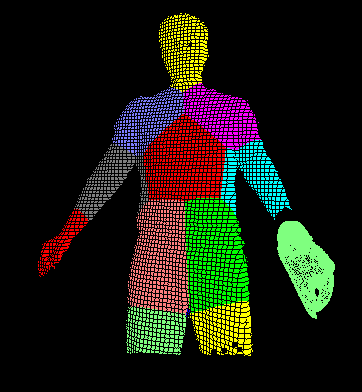
\includegraphics[height=4cm]{image/crabPlier1.PNG} & 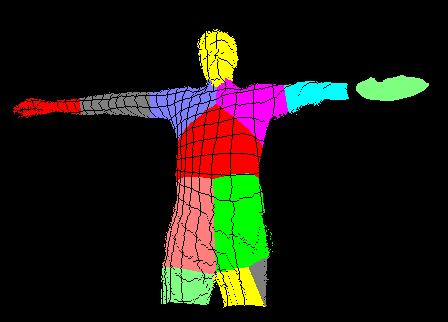
\includegraphics[height=4cm]{image/crabPlier2.PNG} \\
      \hline
      main robot (main gauche) & 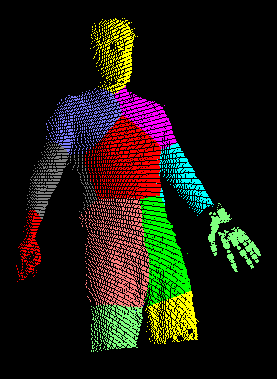
\includegraphics[height=4cm]{image/cyberHand1.PNG} & 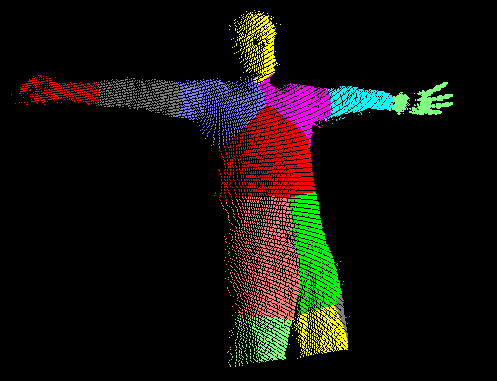
\includegraphics[height=4cm]{image/cyberHand2.PNG} \\
      \hline
      main cybord (main droite) & 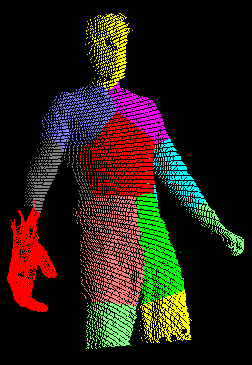
\includegraphics[height=4cm]{image/cyborgHand1.PNG} & 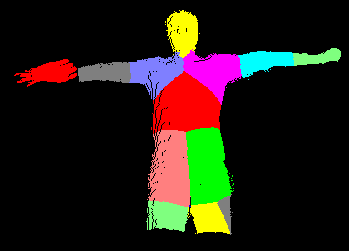
\includegraphics[height=4cm]{image/cyborgHand2.PNG} \\
      \hline
      main de monstre (main droite) & 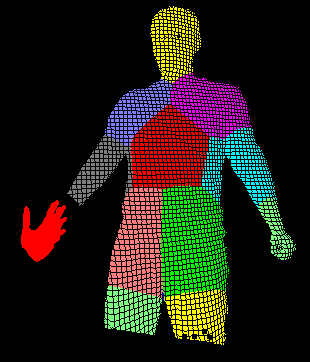
\includegraphics[height=4cm]{image/monsterHand1.PNG} & 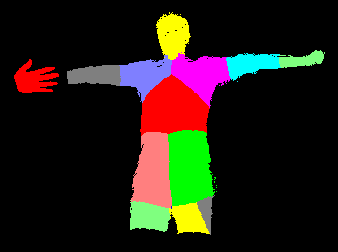
\includegraphics[height=4cm]{image/monsterHand2.PNG} \\
      \hline
      tête cyborg & 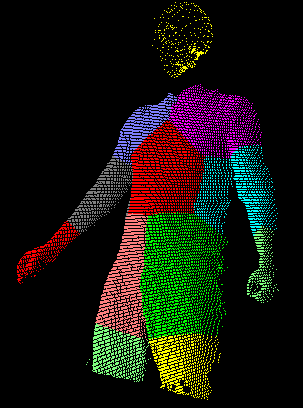
\includegraphics[height=4cm]{image/cyborgHead.PNG} &  \\
      \hline
    \end{tabular}
    \caption{Résultat de remplacement de parties du corps par des modèles 3D}
    \label{tab:modelMatching}
  \end{center}
\end{figure}

Nous pouvons voir sur les résultats de la correspondance de modéle, qu'il y a deux problèmes importants. Le premier problème est celui de l'orientation
de certains modèles 3D. Dans la majorité des tests que nous avons effectué, il y a au moins deux axes sur lequels l'orientation est la bonne. La méthode 
permet de déterminer l'orientation, mais pas le sens, ce qui implique que dans certains cas, l'un des axes soit visuellement tourné du mauvais côté.
Le second problème provient du non raccord du modèle avec le reste du nuage de points, qui est très bien illustré dans l'exemple de la pince de crabe.
Pourtant dans chacun des cas, la translation est juste. Nous le vérifions en comparant la position du centroïde entre le modèle 3D et le nuage de points
(il existe juste un petit décalage sur la profondeur à cause des zones occultées dans le nuage de points). Ce décalage est dû à une différence de ce qui est 
pris en compte comme étant une main (dans les exemples que nous avons vu). Dans le nuage de points, la zone considérée comme étant la main comporte la main et le poignet, alors que 
dans le modèle 3D de la main de monstre le poignet n'est pas présent.\\

Notre méthode serait suffisamment efficace pour remplacer deux nuages de points de membre du corps provenant d'une caméra 3D. On pourrait facilement
remplacer la tête de deux personnes.
Mais la mise en place d'une correspondance entre un nuage de points et un modèle 3D d'une partie du corps n'est pas suffisamment précise. Pour pallier
aux erreurs de l'application, nous avons envisagé de laisser la possibilité à l'utilisateur d'intéragir avec celle-ci. Le plus important est l'orientation
du modèle, et nous savons qu'en cas d'erreur, il faut effectuer une rotation du modèle de 180\degre sur l'un des trois axes. L'utilisateur devrait juste
sélectionner l'axe qui ne convient pas et l'application effectuerait la rotation seule. Maintenant que nous avons vu un cas particulier, nous allons pouvoir
partir sur une application plus généraliste et plus simple en réutilisant ce qui a été vu pour l'application sur le corps humain.  

\subsection{Travaux futures et applications}
L'application que nous avons développé est vraiment la base et de nombreuses extensions peuvent être ajouté.
L'une d'entre elles est la possibilité de bouger la partie du corps modifié en temps réel. Pour l'instant, nous filmons
la scène et l'utilisateur doit mettre en pause l'acquisition lorsqu'il souhaite modifier une partie du corps. Lorsque le
processus est terminé, il serait intéressant de laisser la possibilité à l'utilisateur de relancer l'acquisition afin de
voir la nouvelle partie du corps se deplacer. La possibilité de changer des parties du corps en temps réel durant 
l'acquisition serait un véritable plus, mais la difficulté à optimiser les calcules serait trop important. Sur l'application
actuel, nous sommes à 5 à 10s de calcul pour le remplacement d'une partie du corps.\\

Nous n'avons pas non plus eu le temps de développer l'interface de l'application. Pour l'instant, les modèles de remplacement
sont prédéfinis pour chaque membre, donc l'utilisateur ne peut pas sélectionner le modèle qu'il souhaite.\\

L'un des aspects sur lequel nous avons réfléchi était la construction d'un modèle complet, sans partie occulté, du corps
humain. Cette étape est réalisable avec un algorithme fourni dans le SDK de la Kinect qui est le \og kinect fusion \fg\cite{
KinectFusion}. Cette extension permettrait, en plus d'une simple visualisation de l'utilisateur avec une partie du corps
différente, de reconstruire un maillage complet avec le corps de l'utilisateur. Ce nouveau modèle 3D pourrait alors être
directement utilisé dans un film d'animation ou un jeu vidéo.
